\pagestyle{empty}

\def\widthSqrt{18}
\def\heigthSqrt{25}
\def\smallSubDiv{0.5}
\def\bigSubDiv{1.0}
\def\biggerSubDiv{5.0}

\begin{center}
	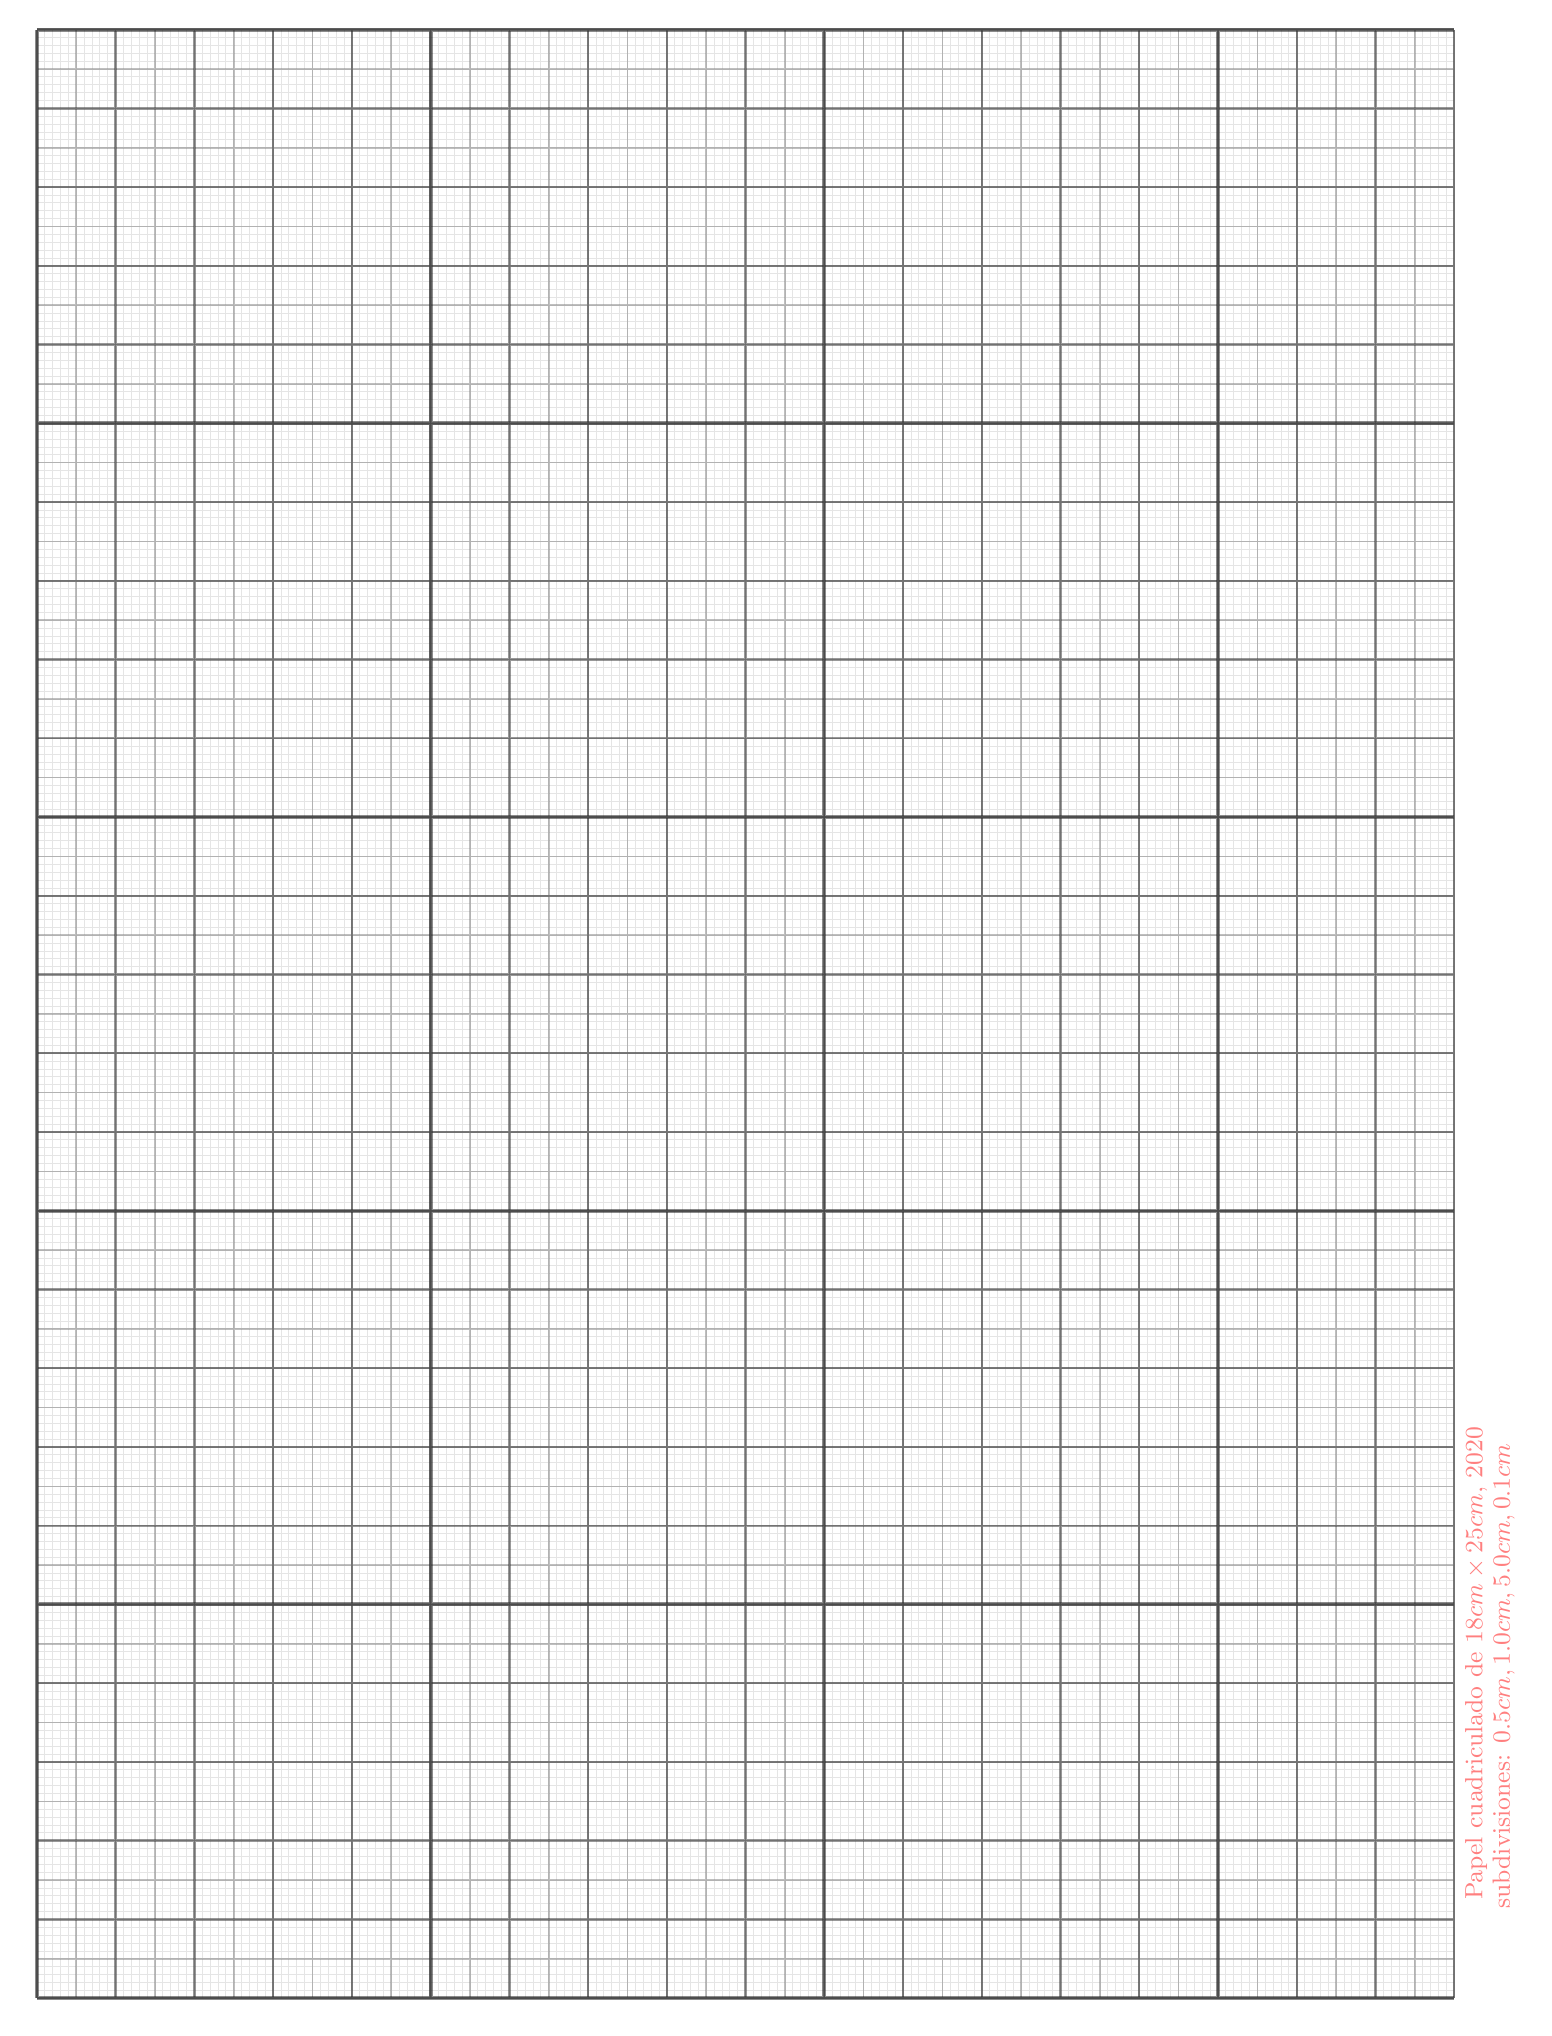
\begin{tikzpicture}[x=1cm, y=1cm, semitransparent]
		\node[] (nodeOne) at (0,0) {};
		\draw[step=1mm, line width=0.1mm, black!20!white] (0,0) grid (\widthSqrt,\heigthSqrt);
		\draw[step=5mm, line width=0.2mm, black!50!white] (0,0) grid (\widthSqrt,\heigthSqrt);
		\draw[step=5cm, line width=0.5mm, black!90!white] (0,0) grid (\widthSqrt,\heigthSqrt);
		\draw[step=1cm, line width=0.3mm, black!80!white] (0,0) grid (\widthSqrt,\heigthSqrt);
		\draw [very thick] (\widthSqrt,1)node[below right,color=red,rotate=90]{ \small{ Papel cuadriculado de $ \SI{\widthSqrt}{cm} \times \SI{\heigthSqrt}{cm}$, 2020}};
		\draw [very thick] (\widthSqrt+0.35,1)node[below right,color=red,rotate=90]{ \small{subdivisiones: $\SI{\smallSubDiv}{cm}, \SI{\bigSubDiv}{cm}, \SI{\biggerSubDiv}{cm}, \SI{0.1}{cm}$}};
		% \def\xi{8cm},
		% \def\yi{8cm},
		% \draw[red,ultra thick,yshift=\yi,xshift=\xi]  (-7.5,0) -- (7.5,0);
		% \draw[red,ultra thick,xshift=\xi,yshift=\yi] (0,-7.5) -- (0,7.5);
	\end{tikzpicture}
\end{center}
